\documentclass[../Main/Knit.tex]{subfiles}

\section{Alzheimer's Disease}

Alzheimer’s disease (AD\nomenclature{AD}{Alzheimer's disease}) is a devastating neurodegenerative disorder, clinically characterised by progressive memory loss, cognitive decline, and behavioural impairment. The most common form of dementia, it is estimated to affect XXX worldwide with numbers expecting to increase to X by 2050, ensuing both a heavy economic and social burden amounting to £XXX each year. Despite international efforts to better understand the disorder for drug discovery and development, there are currently no cure and existing medication only act to reduce symptoms.

\subsection{Pathology}
The symptoms of AD are underpinned by both morphological and molecular changes in the brain. Neuroimaging scans and post-mortem brain analysis from patients reveal significant brain atrophy caused by neuronal and synaptic loss. Further microscopic examination reveal accumulation of beta-amyloid (A$\beta$) in amyloid plaques and aggregation of tau in neurofibrillary tangles (NFT\nomenclature{NFT}{Neurofibrillary tangles}), two key hallmarks of AD, which are now believed to manifest years before presentation of clinical symptoms and diagnosis (\cref{fig:AD_intro}). These neuropathological changes are accompanied with heightened neuroinflammation through abnormal astrocyte and microglial activation.

The progression of these neuropathological changes have been well mapped, particularly the spread of NFTs under the Braak staging\cite{H1991},  with pathology initially apparent in the temporal lobes (hippocampus and entorhinal cortex) and later in the frontal lobes (\cref{fig:AD_development}). Conversely, the occipital lobes, motor cortex, and the cerebellum are relatively resistant to neuronal degeneration even in advanced stages of AD.

\begin{figure}[!htp]
	\centering
	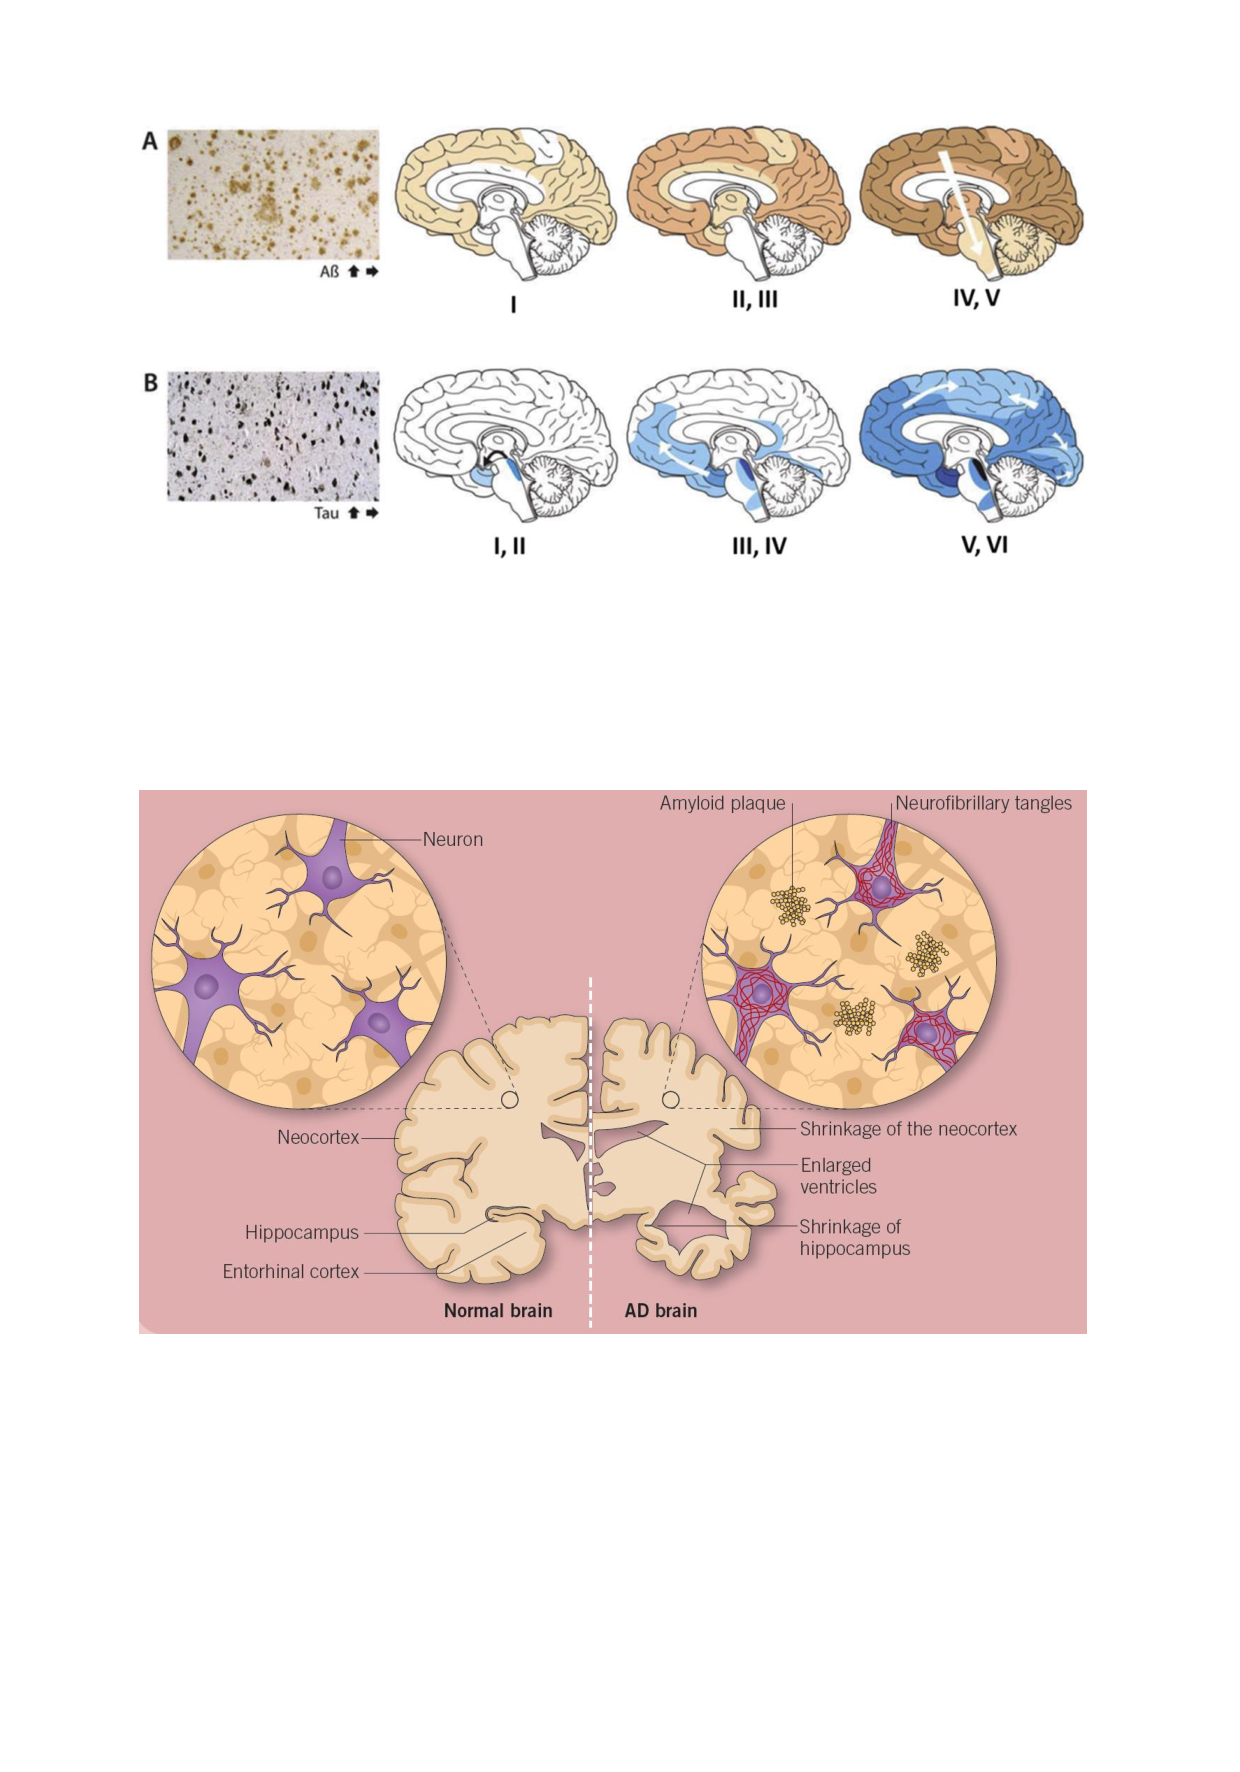
\includegraphics[page=1,trim={0 7cm 1cm 12cm},clip, scale = 0.8]{Introduction_Figures.pdf}
	\captionsetup{width=0.95\textwidth,singlelinecheck=off}
	\caption[Two key hallmarks of AD Neuropathology: amyloid plaques and neurofibrillary tangles]%
	{\textbf{Two key hallmarks of AD Neuropathology: amyloid plaques and neurofibrillary tangles}: Schema comparing a normal healthy brain and a brain with advanced AD. AD pathology is well characterised by the presence of extracellular amyloid plaques and intracellular neurofibrillary tangles, accompanied by significant neuronal loss and subsequent shrinkage of the neocortex and hippocampus. Figure is taken from Palmer (2015)\cite{AlanM.Palmer2015}
	}
	\label{fig:AD_intro}
\end{figure} 

\begin{figure}[!htp]
	\centering
	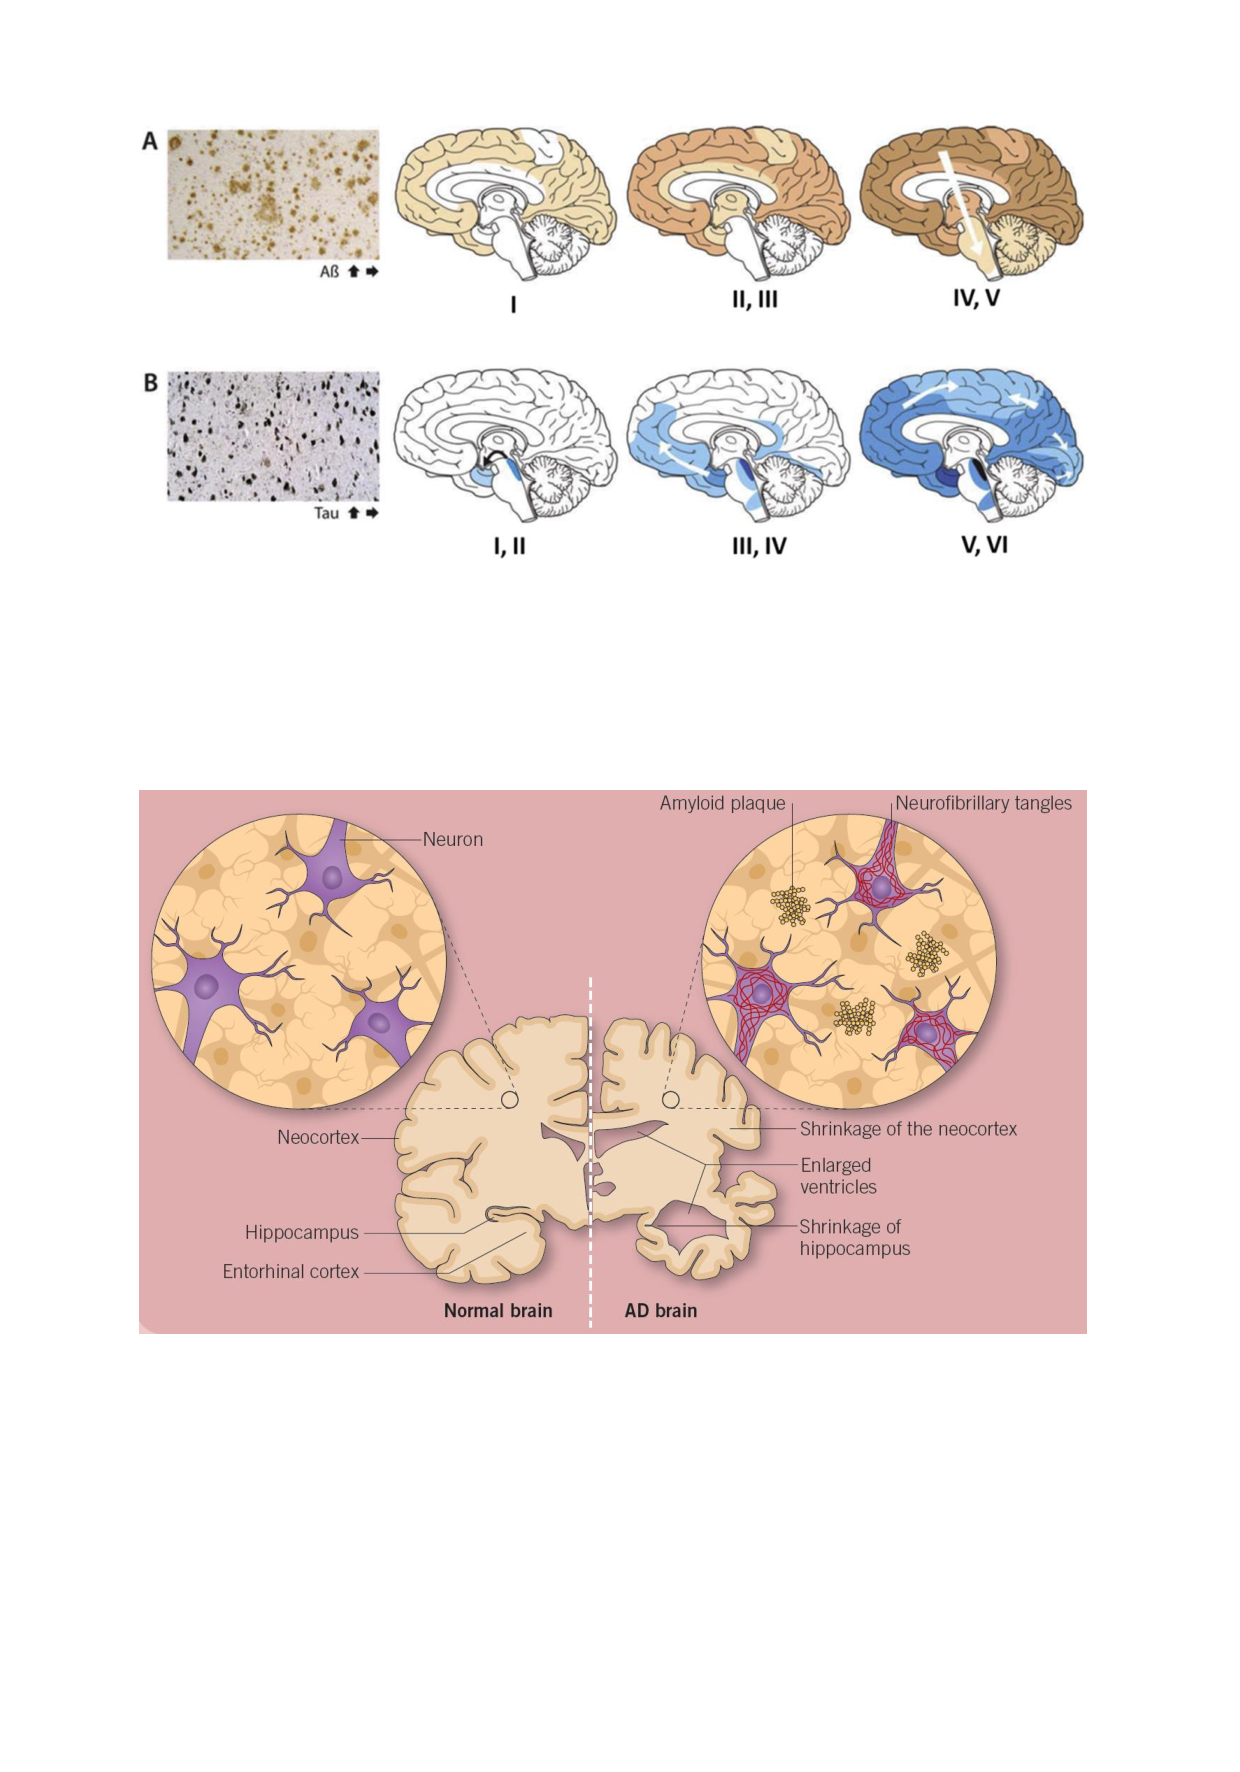
\includegraphics[page=1,trim={0 20cm 0cm 0cm},clip, scale = 0.8]{Introduction_Figures.pdf}
	\captionsetup{width=0.95\textwidth,singlelinecheck=off}
	\caption[Progression of amyloid plaques and neurofibrillary tangles with AD development]%
	{\textbf{Progression of amyloid plaques and neurofibrillary tangles with AD development}: Progression of \textbf{a)} amyloid plaques consisting of A$\beta$ measured according to Thal Phasing\cite{DR2002}, and \textbf{b)} neurofibrillary tangles composed of hyperphosphorylated tau by Braak staging\cite{H1991}. Figure is taken from Jouanne et al.(2017)\cite{Jouanne2017}. 
		\\
		\\ 
		The deposition of A$\beta$ (Figure a) can be mapped with the five stages of Thal Phasing from i) the neocortex, to ii) allocortical regions comprising of the entorhinal cortex and hippocampus, to iii) the striatum, iv) subcortical regions and finally, v) the cerebellum\cite{DR2002}. 
		\\
		\\
		In a similar pattern, the progressive spread of NFTs can be classified under the six stages of Braak (Figure b) from i,ii) the transentorhinal regions such as the entorhinal cortex, to the iii) hippocampus and finally to iv,v) other neocortical regions\cite{H1991}. 	
	}
	\label{fig:AD_development}
\end{figure}

\subsection{Genetics Component}
Although AD is commonly known to affect people aged 65 and above (referred as Late-Onset Alzheimer’s disease, LOAD\nomenclature{LOAD}{Late Onset Alzheimer's Disease}), 5\% of AD cases arise in much younger patients (termed Early-Onset Alzheimer’s disease, EOAD\nomenclature{EOAD}{Early Onset Alzheimer's Disease}) who typically present a clear familial autosomal dominant pattern of inheritance (Familial Alzheimer’s disease, FAD\nomenclature{FAD}{Familial's Alzheimer's Disease})\cite{Jarmolowicz2015}. To date, more than 160 highly-penetrant, causative mutation have been identified in EOAD, all located within three genes involved in amyloid plaque formation: \textit{APP} (amyloid precursor protein\nomenclature{APP}{Amyloid Precursor Protein}), \textit{PSEN1} and \textit{PSEN2} (presenilin 1 and 2\nomenclature{PSEN1}{Presenilin 1}\nomenclature{PSEN2}{Presenilin 2}) \cite{LM2010,Chai2007}. While the clinical manifestations and presentation of neurological hallmarks are similar between EOAD and LOAD, patients with EOAD performed significantly worse in cognitive abilities not involved with memory (such as executive functions, language and visuoconstructional abilities)\cite{Joubert2016}.

Unlike FAD, LOAD does not follow a clear Mendelian inheritance pattern but is rather complex with a heterogeneous genetic composition. Nonetheless, twin studies have reported a relatively high heritability rate of 50-80\% \cite{Gatz2006}, indicating that there is still a large genetic predisposition for developing AD. Indeed over recent years, the emergence of genome-wide association studies (GWAS\nomenclature{GWAS}{Genome-wide association studies}) and subsequent meta-analyses \cite{Bellenguez2020,Naj2020,Kunkle2019,Jansen2019,Lambert2013,Naj2011,Hollingworth2011,Harold2009} have facilitated the identification of multiple genetic loci associated with an increased risk of developing LOAD. These genetic loci are typically changes or variants of single DNA base-pair (single-nucleotide polymorphisms – SNPs\nomenclature{SNP}{Single Nucleotide Polymorphism}) that are more commonly found in individuals with LOAD than without. 

The strongest risk factor for LOAD is the $\epsilon$4 allele of the \textit{APOE} gene \cite{Lambert2013}, which encodes for the cholesterol transporter apolipoprotein E (ApoE) - a key regulator of lipid homeostasis by mediating lipid transport between astrocytes and neurons, a process critical for synaptic function and maintenance\cite{DH2001}. While the $\epsilon$4 allele is estimated to occur in \textasciitilde 15\% of the general population, it is observed in 40\% of patients with AD\cite{Farrer1997,alzgene2010}. Harbouring one APOE$\epsilon$4 allele further increases the risk of developing LOAD by three-four times, while harbouring two $\epsilon$4 alleles increases the risk by 15 times \cite{Farrer1997}. Conversely, the $\epsilon$2 allele confers a neuroprotective effect against AD \cite{Nagy1995,EH1994}. 

The most recent GWAS meta-analysis of 111,326 AD cases and 677,336 control individuals identified 42 significant LOAD risk loci \cite{Bellenguez2020}, many of which were annotated to the non-coding cis regulatory regions of gene (Lambert et al., 2013). These genes included BIN1 (bridging integrator 1\nomenclature{BIN1}{Bridging Integrator }), CLU (clusterin)\nomenclature{CLU}{Clusterin}, CR1 (complement receptor 1\nomenclature{CR1}{Complement Receptor 1}), PICALM (phosphatidylinositol binding clathrin assembly protein\nomenclature{PICALM}{Phosphatidylinositol Binding Clathrin Assembly Protein}), with the most significant genetic locus annotated to APOE (apolipoprotein E\nomenclature{APOE}{Apolipoprotein E}); inheritance of both APOE allele increases the risk of AD development by X\%. Many of these candidate genes fell into established biological pathways\cite{Verheijen2018}: amyloid and tau metabolism, immune response, lipid metabolism, endocytosis, and cell adhesion molecule (CAM) pathways. 

Collectively, these common but low penetrant variants, with the exception of APOE, contribute modestly to the risk of developing AD, highlighting the polygenic nature of AD. The mechanisms behind these variants currently remain poorly understood, however they typically fall into three main biological pathways that may play an important role: the immune system and inflammatory responses, cholesterol and lipid metabolism, and endosomal vesicle recycling. Comprehensive case-control examination of genes proximal to these LOAD-associated variants have further revealed significant differential changes in gene expression and splicing (Humphries et al. 2015), implicating the role of transcriptomic dysregulation in AD pathogenesis. The very fact that most variants lie within the introns rather than exons suggest that it is the fine tune balance of gene expression and regulation that is at play, emphasising the importance epigenomic and transcriptomic studies. 

\clearpage
\subsection{Hypothesis surrounding AD aetiology}
Despite the well characterisation of AD neuropathology, the exact biological mechanisms driving AD onset and pathogenesis are still widely unknown. To date, there are several key hypothesis proposed for the cause of AD: i) amyloid cascade hypothesis, ii) tau tangle hypothesis, and iii) inflammatory hypothesis.

\boldheader{Amyloid cascade hypothesis} 
The amyloid cascade hypothesis posits that the extracellular accumulation of A$\beta$ is the key driver of AD pathogenesis, which initiates a pathological cascade of NFT, cell loss, vascular damage \cite{Hardy1992}. A$\beta$ are short peptides (39-43 amino acids) \cite{J1987} produced from the amyloidogenic cleavage of APP (a transmembrane protein involved in synapse formation and stability) by $\beta$-secretase (BACE\nomenclature{BACE}{Beta-secretase}) and $\gamma$-secretase (a complex protein consisting of PSEN1 and PSEN2) (\cref{fig:APP_Processing}). Due to cleavage at various sites, $\gamma$-secretase produces A$\beta$ of varying lengths: the shorter A$\beta$\textsubscript{40} and slightly longer, but more self-aggregating, A$\beta$\textsubscript{42}. 

In AD, the processing of APP is altered with the vast majority of causative \textit{APP} mutations (typically found at or near the cleavage sites),\textit{PSEN1} and \textit{PSEN2} mutations favouring the production of A$\beta$42 \cite{Li2019,D1996,JT1993}, thereby promoting the formation of insoluble fibrils and plaques characteristic of AD\cite{JT1993}. 

Increasing evidence further postulates that A$\beta$ clearance is regulated in an APOE isoform-dependent manner\cite{Castellano2011} with APOE4 having low binding affinity to A$\beta$ and thus, being the least efficient at A$\beta$ clearance\cite{RM2012} - carriers of $\epsilon$4 allele have more pervasive amyloid plaques than non-carriers\cite{DE1993,E2009}. Furthermore, APOE4 is poorly lipidated compared to APOE2 and APOE3, resulting in increased propensity to aggregate\cite{DM2006} - of note, lipidation is mediated by ABCA1\cite{R2010}.
%https://www.nature.com/articles/nrn2620

%Although interestingly, the neuroprotective ApoE$\epsilon$2 allele while associated with intact cognition is also associated with AD pathology in the oldest old population\cite{DJ2009}, suggesting that an A$\beta$-independent mechanism may be at play.   
    
\boldheader{Tau tangle hypothesis} 
The tau hypothesis posits that the phosphorylation and aggregation of tau to form NFTs are the primary drivers of AD\cite{KS1986}, which is also the defining feature of more than 20 other neurodegenerative disorders known collectively as tauopathies\cite{Orr2017}. Tau, encoded by \textit{MAPT}, is a microtubule-associated protein involved in microtubule maintenance and stability.. It is thought that in AD, the increased phosphorylation of tau induces detachment from microtubule and promote aggregation of paired helical filaments that disrupt microtubule function and subsequent axonal growth and transport. The severity of NFTs has shown to correlate better with cognitive decline and progression of AD than amyloid plaques \cite{Serrano-Pozo2016,Giannakopoulos2003,PV1992} with its spread traced through Braak staging \cite{H1991}(\cref{fig:AD_development}\textbf{b}).  

\begin{figure}[!htp]
	\centering
	\includegraphics[page=2,trim={0 15cm 0cm 0cm},clip, scale = 0.8]{Introduction_Figures.pdf}
	\captionsetup{width=0.95\textwidth,singlelinecheck=off}
	\caption[Cleavage of APP into A$\beta$ by $\beta$-secretase and $\gamma$ secretase]%
	{\textbf{Cleavage of APP into A$\beta$ by $\beta$-secretase and $\gamma$ secretase}: Schema depicting sequential cleavage of APP, a transmembrane protein, by $\beta$-secretase and $\gamma$-secretase, which can produce A$\beta$ of varying lengths with varying propensities to oligomerise and aggregate. Figure is taken from Makin (2018)\cite{Makin2018}. 
	}
	\label{fig:APP_Processing}
\end{figure}

\subsection{Mouse Models}
%https://molecularneurodegeneration.biomedcentral.com/articles/10.1186/s13024-017-0231-7
%Molecular changes in both genes and regulatory regions are highly conserved between human AD and mouse model neurodegeneration. 
With autosomal dominant mutations predominantly residing in \textit{APP}, \textit{PSEN1}, \textit{PSEN2}, expression of these human AD-associated genes in mouse have been the foundation of most AD mouse models. 
Mouse models based on transgene insertion of \textit{APP}, typically harbouring the double swedish mutation at the beta-secretase cleavage site, develop significant amyloid pathology corresponding to increased A$\beta$ production and exhibit memory loss, though neuronal loss is not observed \cite{Hall2012}. Mouse models with \textit{PSEN1} mutations and insertion of human \textit{APP}, unsuprisingly progress much more quickly with amyloid pathology and behavioural deficits. 5XFAD mice exhibit neuronal loss that are not observed in other mouse hAPP or hAPP/PS1 models. 
AD-associated tau pathology is recapitulated by expression of transgenic human tau, harbouring mutations that cause frontotemporal dementia (FTD).  

It is important to note that there are currently no mouse model that encapsulates all the defining features of AD and one of the major criticisms of current AD mouse models us how representative they are of sporadic, late-onset AD. Since my PhD, there have been efforts to generate mouse models that more closely resemble LOAD with incorporation of AD-associated variants, such as $\epsilon$ variant of \textit{APOE} 


Nonetheless, AD mouse models act as a useful reductionist tool to dissect and understand the facets that drive AD-associated pathology and developments \cite{Hall2012}. 

\subsection{Currently available mouse models in AD}

\pagebreak
\section{Gene expression and regulation}

Common observation from gene expression analysis is that genes typically express multiple isoforms, and the greater the number of annotated isoforms, the greater the number of expressed isoforms (with a plateau of 12 isoforms) \cite{Djebali2012}. These isoforms are defined as mRNA transcripts that are transcribed from the same gene locus, but generated and processed in a different manner either through alternative transcriptional start sites (Alternative transcription initiation (ATI) \nomenclature{ATI}{Alternative Transcription Initiation}), alternative polyadenylation sites (APA) \nomenclature{APA}{Alternative Poly-Adenylation} or alternative splicing (AS) \nomenclature{AS}{Alternative Splicing}). However, as most studies are performed on bulk-tissues, it is unclear whether this is a consequence of multiple isoforms in one single cell or from multiple isoforms from multiple single cells. Perhaps assumed but the expression of alternative isoform is also not consistent, with usually a dominant isoform \cite{Djebali2012}.

MicroRNA \nomenclature{miRNA}{micro RNA}), 22 nucleotides long, involved in regulation of gene expression through various ways, including promotion of transcript degradation and inhibition of translation machinery. This is typically achieved by the contact of miRNA with the 3'UTR of mRNA. It is estimated that up to XX\% of genes are regulated by miRNAs, and has been found to multiple roles in immune functions.

\pagebreak
\section{Transcriptional profiling}
Transcriptome profiling by the identification of full landscape of transcribed elements is critical to elucidate the functional relationship between the genomic loci and molecular mechanisms that drive development and diseases. Transcriptome profiling of disease-relevant tissue has enabled discovery of pathogenic coding and non-coding splicing variants in rare diseases, that would have otherwise been missed by exome and whole-genome sequencing in Mendialian disease diagnosis (\cite{Cummings}, \cite{Kremer2017})
	
With Mendialian diseases such as Duchenne muscular dystrophy, pathogenic variants that result in aberrant splicing (exon inclusion, exon skipping, exon extension, intronic splice gain, exonic splice gain) can have significant downstream impacts (i.e. loss of function). A genetic variant can result in aberrant splicing in the following ways (\cite{Cummings}):
\begin{itemize}
	\item variant at the splicing donor or acceptor site resulting in a masked splicing site and downstream alternative site used for splicing, thus exonic extension
	\item variant at the splicing donor or acceptor site resulting in masked splicing site, exon skipping
	\item variant within an intron (cryptic splice site), resulting in a strong splicing site and thus intronic splice gain
	
\end{itemize}

\subsection{Alternative Splicing}
Alternative splicing and polyadenylation is a widespread phenomenon that facilitates generation of multiple distinct mRNA transcripts or isoforms from one gene, which are subsequently translated to different protein isoforms with unique, and potentially, antagonistic functions \cite{Wang2008}. AS further regulates gene expression through various mechanisms: non-sense mediated decay, miRNA-mediated mRNA degradation, altered translational efficiency of isoforms. In contrast, alternative polyadenylation regulates RNA transportation, localization, stability, and translation by generating splice isoforms with different cleavage sites.

Alternative splicing is essential in shaping transcriptome and proteome diversity - over 95\% of 22,000 protein-coding multi-exonic human genes are estimated to undergo alternative splicing \cite{Pan2008}, with up to 70\% containing multiple polyadenylation sites and 60\% with two or more promoters from alternative transcription start sites \cite{Carninci2006}. Each gene is estimated to have on average six transcript isoforms \cite{Dunham2012}, and this figure is likely to increase with more transcriptomic studies. It occurs most prevalently in the brain implicating its role in neuronal development and maintenance (Pan et al., 2008) (Mazin et al., 2014) (Raj, Blencowe, 2015). It is predicted that a single cell, with a transcription of 600,000 molecules, will have generated 5 - 15 conservative isoforms per gene, and 2-4 exon cassette isoforms (\cite{Karlsson2017}) (a single oligodendrocyte contained ~2000 conservative transcripts associated with 700 genes, and 1000 unique isoforms). 


\boldheader{Mechanism}
% summary: https://www.cell.com/current-biology/pdf/S0960-9822(14)01553-X.pdf
Nuclear pre-mRNA splicing involves the removal of non-coding sequences (introns) from the mRNA precursors and ligation of coding sequences (exons). This relies on a concerted and regulated assembly of the spliceosome - a multimegaton, dynamic ribonucleoprotein complex - by its recognition and stepwise-bindingo sequence elements within the pre-mRNA (cis-elements), and a group of regulating splicing factor proteins (trans-elements). There are two types of spliceosome - major and minor - both of which involve the activity of five uridine-rich small nuclear ribonucleoproteins (snRNP\nomenclature{snRNPs}{Small Nuclear Ribonucleoproteins}) and numerous non-snRNP proteins\cite{Will2011}. Using a similar mechanism but composed of different snRNPs, the minor spliceosome removes less than 1\% (0.4\%) of introns\cite{Turunen2013} and is thus referred to as "U12-dependent non-canonical splicing", as opposed to "U2-dependent canonical splicing" with major spliceosome.

Correct splicing first requires the recognition of short sequence motifs upstream (5' splice site - 5'SS\nomenclature{5'SS}{5' Splice Site} - or donor site) and downstream (3' splice site - 3'SS\nomenclature{3'SS}{3' Splice Site} - or acceptor site) of the intron/exon boundary and the branch point sequence\cite{Aebi1986,Lamond1987} (BPS\nomenclature{BPS}{Branch Point Sequence}  (Figure \ref{fig:AS_mechanism}a). The 5'SS is typically defined by a conserved nine-nucleotide sequence that predominant contains a GU(T) dinucleotide, whereas the 3'SS is defined by a variable length polypyrimidine tract (PPT\nomenclature{PPT}{Polypyrimidine Tract}) followed by a conserved AG dinucleotide \cite{Will2011}. Almost all introns in both human and mouse are flanked by the GT-AG splice site dinucleotides\cite{Sheth2006} (termed splice junctions), with other variations such as GC-AG and AT-AC known to exist in very minute proportions; GC-AG and AT-AC comprises \textasciitilde0.9\%\cite{Parada2014} and \textasciitilde0.09\%\cite{Parada2014} of human splice sites and are processed by the major and minor spliceosome, respectively. The branch point sequence is defined by a highly conserved sequence, distinguished by an adenosine, and is typically found within 18-40 nucleotides upstream of the 3'SS \cite{Will2011}. 

In the classic splicing model (Figure \ref{fig:AS_mechanism}), spliceosome assembly first involves the identification of 5' and 3' splice sites, followed by sequential assembly of the spliceosome components as the spliceosome matures and activates for catalysis\cite{Herzel2017} - intron excision is primarily executed by two transesterification reactions. Recent studies suggest that this process occurs co-transcriptionally, such that the intron can be identified and removed as soon as it is synthesised by the RNA polymerase (Pol II). 

\begin{figure}[!htp]
	\centering
	\includegraphics[page=3,trim={0 14cm 8cm 2cm},clip, scale = 0.8]{Introduction_Figures.pdf}
	\captionsetup{width=0.95\textwidth,singlelinecheck=off}
	\caption[Splicing Mechanism: spliceosome assembly on nascent RNA]%
	{\textbf{Intron removal is catalysed by the assembly and complex rearrangement of spliceosome. a)}:  Consensus sequence of splice sites that demarcate the intron/exon boundary and are essential for recruitment of spliceosomal snRNPs. \textbf{b)} Co-transcriptional assembly of spliceosome with stepwise interaction of spliceosomal snRNPs, with the formation of 
	\begin{enumerate}
	\item E (Early) commitment complex with the identification and binding of U1 snRNP to the 5'SS and branchpoint binding protein (BPP\nomenclature{BPP}{Branchpoinnt Binding Protein} to BPS 
	\item A (Assembly) catalytically-active complex with association of U2 snRNP to the branch site following the dissociation of BPP. The "A" here denotes to the adenosine of BPS
	\item B pre-catalytic spliceosome complex with recruitment of U4,U5 and U6 snRNPs
	\item Bact pre-catalytic spliceosome complex after major conformational rearrangements within the spliceosome (RNA-protein and RNA-RNA interactions) followed by the release of U1 and U4 snRNP to expose the adenosine from BP to the 5'SS 
	\item B* catalytically-active complex with nucleophilic attack of adenosine on 5'SS (first step of transesterification) 
	\item C catalytically-active complex with further conformational changes in the U2 snRNA to C* complex, with nucleophilic attack of the 5'SS to 3'SS (second step of transesterification) 
	\item P (Post-spliceosome complex). The mRNA product is then released from remaining spliceosome (ILS), now bound to the intron lariat. The snRNPs can then disassociate and be recycled for next cycle of splicing.
	\\
	\end{enumerate} 

	BPS - Branch point sequence, CTD - carboxyl-terminal domain, ILS - Intron lariat spliceosome, PAS - poly(A) site, SS - Splice site, TSS - Transcription start site,TTS - Transcription termination site. Figure is taken from Herzel et al. 2017\cite{Herzel2017}.
}
	\label{fig:AS_mechanism}
\end{figure}


\boldheader{Events}
Isoforms can differ at the 5' (alternative transcript start sites - TSSs), exons (alternative splicing) and 3' end (alternative transcription termination sites - TTSs)). Exon splicing can be further divided into alternative splice sites (alternative 5'-splice site, alternative 3'-splice site), exon skipping and intron retention. 
AS events can be classified into five different types: 
\begin{itemize}
	\item Intron retention \nomenclature{IR}{Intron Retention}, defined by the presence of an exon which overlaps with the intron of another transcript within the same gene. IR can introduce stop codons, subsequently prompting non-sense mediated decay but can also change open reading frame \nomenclature{ORF}{Open Reading Frame}, generating functionally different variant 
	\item Skipped exon \nomenclature{SE}{Skipped Exon}, defined by the presence a missed exon which is completely overlapped with an intron of another transcript 
	\item Alternative 5' splice site \nomenclature{A5SS}{Alternative 5' Splice Site}
	\item Alternative 3' splice site \nomenclature{A3SS}{Alternative 3' Splice Site}
	\item Mutually Exclusive Exon 
\end{itemize} In addition to above five common categories, many other complex types, such as alternative position, i.e., alternative 3' and 5' site (Wang and Brendel, 2006), AS and transcriptional initiation (ASTI) (Nagasaki et al., 2006) alternative first exons (Chen et al., 2007), and composite patterns (Wang and Rio, 2018), can occur."

\newpage
\textbf{Nonsense mediated decay (NMD)} \nomenclature{NMD}{Nonsense Mediated Decay} products are alternatively spliced isoforms that are not translated into proteins, by containing an early stop codon. A premature termination-translation codon highly supportive of NMD is defined by a stop codon within at least 50-55 base pairs upstream of splice junctions. 

\textbf{Fusion Transcripts} are a consequence of trans-splicing event of merging two separately encoded pre-mRNA into one transcript

\textbf{Long non-coding RNA \nomenclature{lncRNA}{Long non-coding RNA}} are polyadenylated RNA with more than 200 nucleotides. 
	
\textbf{Natural Antisense Transcripts \nomenclature{NATs}{Natural Antisense Transcripts}} 

\textbf{3'Polyadenylation} Polyadenylation of 3'end of mRNA regulates mRNA stability and translation efficiency. Studies using long-read sequencing of human transcriptome have revealed differences in poly(A) length distribution between genes, and even between isoforms of the same gene  with protein-coding isoforms having shorter poly-A tails than intron-retaining isoforms (\cite{Workman2019a}. This is line with studies showing that hyperadenylation targets intron-retaining transcripts for degradation (\cite{Bresson2015})

\textbf{Allele-specific expression} Preferential transcription of RNA from the paternal or maternal copy, which can be assessed using long-read sequencing from coverage of heterozygous SNP. 

\subsection{Short-read RNA-sequencing}
\label{rnaseq_intro}
Transcriptomic profiling of AD in human and mouse models (determination of changes in splicing patterns) have been traditionally performed using exon microarrays and more recently, RNA-Sequencing (RNA-Seq\nomenclature{RNA-Seq}{RNA-Sequencing}) (Table X).
Multiple methods for transcriptome profiling in the past: 
\begin{itemize}
	\item One of the first methods of transcriptome profiling is to use multiple expressed sequence tags (EST) \nomenclature{EST}{Expressed Sequence Tags}), short oligonucleotide tags, that can be sequenced - Serial Analysis of Gene Expression \nomenclature{SAGE}{Serial Analysis of Gene Expression}).
	\item Hybridisation of cDNA to oligonucleotides on an array (microarray) i.e Affymetrix's GeneChips, also allowing examination of individual exons
	\item Quantitative PCR for validation of expression data 
\end{itemize}

Through massively-parallel sequencing of amplified DNA templates in a “sequence-by-synthesis” fashion to generate short-reads (Figure X) rather than relying on hybridization of target and probe, RNA-Seq allows deep surveying of the entire transcriptome, with transcript identification and quantification, and interrogation of alternative splicing events by discovery of splice variants and polymorphisms. With greater signal-to-noise ratio and higher nucleotide-level resolution, has been effective in identifying AS events such as exon skipping and intron retention, with the establishment of its role in diseases (E. T. Wang et al., 2008). 

Typically, several millions of short reads (ranging in length between 200bp - 700bp depending on the sequencing platform) are generated and aligned to genome to identify transcribed sequences. Major advances, including generation of reads that retain information on transcript orientation, allowing input of low yield or quality, have revolutionised the field. Also, now possible to sequence transcriptome \textit{de novo}, allowing characterisation of novel organisms. 

However, despite its power to identify and quantify gene expression (transcriptional profiling at a gene level) even with paired-end sequencing of both ends of a library fragment, RNA-Seq is severely limited in assembling and reconstructing transcripts due to the reliance of short-reads that are only able to span a small part of the transcript rather than the full length (Figure X) \cite{Gordon2015}\cite{Wang2016}; short reads have an average length of 100-500bp, whereas transcripts are on average 2-3kb - 50\% of human transcripts are > 2.5Kb \cite{Sharon2013} and ranges from 60bp to 103kb \cite{Piovesan2016,Sharon2013} - the longest known human processed transcript to date is Titin with 363 exons and spanning 106kb \cite{Bang2001}. In particular, there are three transcriptional features that are difficult to characterise with short reads \cite{Kuo2017}:
\begin{enumerate}
	\item Transcript start sites (TSS) \nomenclature{TSS}{Transcription Start Sites} and Transcript termination sites (TTS) \nomenclature{TTS}{Transcription Termination Sites},for which any interior multiple TSS and TTS sites within a transcribed locus would be undetected due to overlapping exons and splicing junctions, and low coverage  
	\item Exon chaining given that short-reads typically only span one splice junction. Thus, while short-reads may able to accurately identify the exons present, the exact sequence and linking of the exons are predicted by short-read assemblers with challenges (Figure \ref{fig:kuo_splicing}).  
	\item Transcriptional Noise, particularly of reads in intronic regions that are falsely identified as intron retention, or of reads in intergenic regions that are erroneously classified as fusion gene. 
\end{enumerate}
It is therefore unclear which combination of exons are spliced in, and whether alternative (distant) exons pairs are included in mutually exclusive or independent fashion (i.e. whether events are coordinated though some distant alternative exons have shown to be correlated included (\cite{Fagnani2007})Furthermore, short-read RNA-sequencing fails to capture the connectivity of exons and informs whether the alternative processive events are coordinated (coordination is defined by two or more alternative RNA processing events are dependent of each other and the probability of this occurrence is greater than the observation of the sole event). --> Molecular co-association of distant human alternative exons


\iffalse
\begin{figure}[h]
	\centering
	\vspace{20pt}
	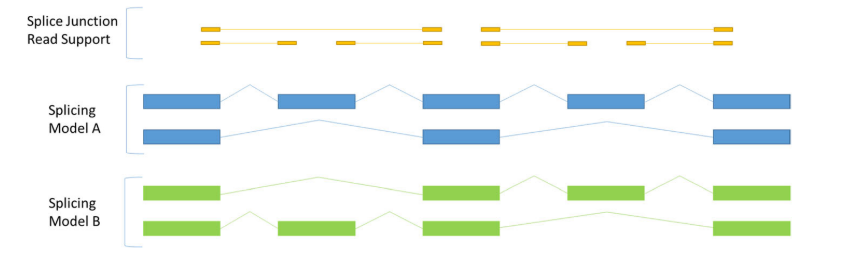
\includegraphics[width=0.8\linewidth, height=0.2\textheight]{Pictures/kuo_splicing_picture.png}
	\captionsetup{width=0.95\textwidth}
	\caption[Challenges of using short-reads for transcript assembly]%
	{\textbf{Challenges of using short-reads for transcript assembly}: Example of a transcript model that is impossible to resolve using short-reads (yellow). Figure and caption taken from \cite{Kuo2017}}
	\label{fig:kuo_splicing}
\end{figure}	
\fi
Various bioinformatic packages have been developed to assemble these short reads into transcripts, by probabilistically assigning and mapping reads to isoforms and exon-exon boundary or XXX, to identify and estimate transcript abundance (Figure X) (Trapnell et al., 2010)(Kingsford, Schatz, \& Pop, 2010)(Au et al., 2013). This, however, requires complex computational analysis and has resulted in conflicting outcomes and limited success, compounded by the fact that alternative transcripts often have significant overlaps and only a minor proportion of reads span splicing junctions. These tools further rely heavily on reference annotation libraries (RefSeq/Ensembl) or predefined splicing events, which may be inaccurate or incomplete; resulting in prediction of transcripts that do not exist (false positives) or fails to detect true transcripts (false negatives) particularly with genes that have large number of variants (Au et al., 2013). Pre-defined models are particularly limiting when comparing splicing profiles between different conditions, such as control versus transgenic mice, as any splicing changes observed are likely to be AD-specific. While there are tools that are de novo, these typically generate different and often conflicting results [Table X]. 

Attempts to overcome challenges with transcriptome assembly included generation of “synthetic long reads”, by tagging full-length complementary DNAs with unique molecular identifiers (UMIs) before cluster amplification and sequencing on Illumina (Tilgner et al., 2015). With the presence of UMIs, transcript isoforms can be reconstructed for up to 4Kb for isoform discovery and expression analysis (Stark, Grzelak, \& Hadfield, 2019). [However…]
RNA-Seq is thus impaired to profile the transcriptome at an isoform-level, investigate cis-acting mechanisms with transcripts, and characterise the functional aspects of isoform diversity (Tardaguila et al., 2018)(Hayer et al., 2015).

\subsection{Long-read sequencing approaches}
The limitations with RNA-Seq were addressed with the emergence of long-read, third-generation sequencing approaches, which generated longer reads that were able to span the full-length transcript. Rather than massively-parallel sequencing of templates in “wash-and-scan” fashion that resulted in de-phasing and subsequently shorter reads, both platforms allowed real-time sequencing of templates in an uninterrupted and processive manner. Two technologies currently dominate this space: Single Molecule Real Time (SMRT\nomenclature{SMRT}{Single Molecule Real Time}) from Pacific Biosciences (PacBio \nomenclature{PacBio}{Pacific Biosciences}) and protein nanopore sequencing technology from Oxford Nanopore Technologies (ONT \nomenclature{ONT}{Oxford Nanopore Technologies}). Both platforms have been able to generate very long reads (\textasciitilde15kb for PacBio and >30kb for ONT). The performance and cost specifications of these two platforms are outlined in Table X. Other long read sequencing methods and protocols, synthetic long read (SLR \nomenclature{SLR}{Synthetic Long Read}) (\cite{Tilgner2015}) or sparse isoform sequencing (spISO-seq \nomenclature{spISO-seq}{Sparse Isoform Sequencing}) (\cite{Tilgner2018}), however these require more complex workflows.

The consequent generation of longer reads, ranging from 300 – 20,000 bases provided unprecedented ability to sequence entire or new entire lengths of transcripts from 5’ end to polyA tail, relinquishing the need for transcriptome assembly and resolving splicing junctions. Allowing greater accuracy at transcript identification, an increasing number of studies have used such technologies to characterise isoform diversity and splicing with unprecedented success (Table X). Generally in comparison with RNA-Seq, Iso-Seq encapsulates longer transcripts, identifies novel gene locus, and correction of gene model. "Long transcript reads provide better support and higher accuracy in splice junctions than short reads, when these reads are aligned back to the genome. Thus gene models predicted from long reads yield more accurate exon/intron structure and can merge two or more misannotated adjacent genes."


\subsection{Hybrid approach of short and long read sequencing}
Despite the ability of long-read sequencing (particularly, Iso-Seq\nomenclature{Iso-Seq}{Isoform Sequencing}) to discover large number of novel and longer transcripts and identify complex splicing events such as alternative adenylation, there are inherent biases to sequencing the more highly-expressed and relatively shorter transcripts. Consequently, while the new chemistry has improved the error rate and increased throughput, the coverage is still insufficient for accurate transcript quantification and sensitive differential transcript analysis based on long reads alone (Koren et al., 2012). Furthermore, there is currently no consensus to validate or functionally characterise these transcripts (B. Wang, Kumar, Olson, \& Ware, 2019). The current standard for such application is thus a hybrid approach of aligning the short-reads to the long-reads to improve alignment and assemblage, and for downstream isoform quantification. 

\subsection{Isoform quantification} 
Isoform-specific expression can be deduced from short-reads alone using statistical models if the gene is well annotated (i.e. all isoforms are known) based on i) reads aligning to contiguous genomic segment (exonic reads) and ii) reads aligning to two contiguous segments with a single gap of 60-400bp (junction reads)(Jiang and Wong, 2009)).

Various bioinformatic tools and computational models have been developed to quantify isoform quantification from RNA-Seq data. There are currently two main methods:
\begin{enumerate}
\item Inclusion level, calculated for a regulated exon by aligning reads either to candidate alternative exons and its junctions (inclusion reads), or to flanking exons and subsequently skipping the candidate alternative exon (skipping/exclusion reads) (Chen et al. 2012)
\item Percent-Spliced-In (PSI\nomenclature{PSI}{Percent-Spliced In}), calculated by proportion of isoforms that include the exon (Venables et al. 2008)(Katz et al. 2010). If the PSI value is calculated for a particular splicing event, it can be considered equivalent to the inclusion level. 
\end{enumerate}
Isoform quantification can either be expressed as a global measure of expression, which provides a global gene expression ranking in one sample (measured by RPKM: Reads of a transcript sequence per Millions mapped read\nomenclature{RPKM}{Reads of a transcript sequence per Millions}), or as a relative measure of expression, which is normalized per gene locus and comparable across conditions (measured by inclusion level or PSI value). 

Isoform abundance calculated by aligning short-reads to transcriptome is preferential to alignment with reference annotation library (RefSeq/GENCODE) in narrowing down the isoforms expressed and thus subsequently enabling more reliable abundance quantification. Reference annotation library is constructed on all data from the same species, and inclusion of annotated but not truly expressed isoforms can increase variability of abundance estimates. Finally, if the reference library is incomplete, then truly expressed isoforms would be completely missed and RNA-Seq reads would be incorrectly assigned to annotated isoform (\cite Au2013)


\textbf{Differential Isoform Usage }\\
\label{intro:dtu}
When analyzing splicing patterns between multiple conditions, changes in isoform abundance can be defined in two ways: 
\begin{enumerate}
	\item Differential Isoform Expression (DIE\nomenclature{DIE}{Differential Isoform Expression}): changes in absolute expression of an isoform, evaluated using count matrixes 
	\item Differential Isoform Usage (DIU\nomenclature{DIU}{Differential Isoform Usage}): changes in relative expression of an isoform from the same gene, resulting in a change in isoform proportion and is evaluated using changes in gene exon usage	
\end{enumerate}

Figure X shows an example of a change in DIE but no change in DS: A two-fold increase of both isoforms from the same gene results in a change in absolute but not relative expression to one another. A change in DIE but not in DS may indicate a transcription-related mechanism. If a change in DS is observed, a change in DIE of one of the isoforms would also be observed. A change in multiple isoforms would also be observed, as long as the change is not in the same direction (upregulated/downregulated) with the same magnitude. Any changes in DS/relative abundance of isoforms indicate a splicing-related mechanism. 

In addition to exploring differential splicing in terms of isoform abundance, which typically involves an exon-based approach that focuses on differential exon usage (i.e. DEXSeq), a splicing based approach can also be taken. This involves analyzing individual splicing events (exon skipping, alternative donor and acceptor) for systematic changes between conditions. rMATS, SUPP2, LeafCutter and Majiq are such tools that identify and quantify splicing events using junction reads. 

Applications of these novel bioinformatic approaches to study alternative splicing in AD human post-mortem brains revealed over 2000 genes with differential transcript usage, including \textit{APP} and \textit{BIN1} \cite{Marques-Coelho2021}.


\section{Aims and Objectives}
\begin{enumerate}
	\item Whole transcriptome analysis of AD post-mortem brain tissues as reference dataset, shed light on differential isoform expression
	\item Particular interest on 19 loci identified from meta-analysis of GWAS studies on AD (Lambert et al. 2013) Targeted transcriptome analysis  
	\item Classification of AS events, which most commonly observed/dominant? Isoforms derived from transcriptional regulation (alternative promoters) vs post-transcriptional regulation? 
	\item Impact of AS events on protein domains. Non-sense mediated decay? 
	\item Integration with other (epi)genetic analysis on same samples, i.e. DNA methylation, lysine acetylation, gene expression 
	\item Protein analysis? Integration with any publicly available mass-spec datasets 
\end{enumerate}

\begin{figure}[htb]
	\begin{center}
		\includegraphics[page=3,trim={2cm 35cm 0 2cm},clip,scale = 0.55]{Introduction_Figures.pdf}
	\end{center}
	\captionsetup{width=0.95\textwidth}
	\caption[Mouse samples for Whole and Targeted Transcriptome Iso-Seq]%
	{\textbf{Mouse samples for Whole and Targeted Transcriptome Iso-Seq}.}
	\label{fig:samples}
\end{figure} 

Gene expression and mRNA isoforms vary widely across tissues (\cite{Wang2008}), thus sequencing the disease-relevant tissue (in this case entorhinal cortex) is important for understanding the pathology of AD. However, it is consequently important to note that other tissues may have to be considered to fully grasp the whole picture of AD development. 

While human post-mortem brain tissues remain to be the gold standard for transcriptomic studies, important to highlight that post-mortem interval and storage conditions of brain material highly influence transcriptome stability, particularly affecting alternative splicing. Furthermore changes in gene/transcript expression can be due to differences in cellular composition (i.e. neuronal loss/reactive gliosis) rather than indicative of disease-associated transcriptional regulation. 

\section{Future Directions}
At the time of writing, there have been other major advances in the field have unfortunately not be explored. This include, single cell transcriptomics and Direct RNA-Sequencing. Analysis of mRNA expression at the resolution of individual, "single", cells, allowing representation of cell-to-cell variation rather than taking the stochastic average from bulk measurements, and thereby resolving heterogeneity. This is currently achieved by the capture and analysis of single cells using a microfluidic or droplet-based technology. Importance of single cell approaches highlighted in \cite{Karlsson2017} with few isoforms shared between cells (7\% of all detected isoforms shared between all cell-types, though this increased to 60\% for exon-cassette isoforms). 

To date, Direct RNA sequencing of the native RNA molecules rather than the cDNA is only possible on the ONT. This approach offers several benefits over standard cDNA sequencing, in i) eliminating the risk of generating library artefacts from reverse transcription and PCR, ii) removing length bias toward shorter abundant fragments that could skew the population of transcripts, and finally iii) elucidation of RNA epigenetic modifications. 

Single-cell studies have highlighted the difference in transcriptome diversity at a single cell level, with small overlap of isoforms between cells (\cite{Karlsson2017}). Previous methods on quantifying transcripts at a single cell level have relied on RNA-fluorescence in-situ Hybridisation (RNA-FISH), which is limited in terms of throughput and characterisation of complex splicing events (\cite{Byrne2017})

While the methods I have adopted for long-read sequencing in this thesis allows interrogation of full-length transcripts, this is reliant on the generation and amplification of cDNA from mRNA, which can produce artefacts (template switching), introduce bias (distortion of relative cDNA abundance) and lose RNA modifications. In 2018, ONT showed that it was able to sequence RNA directly using the minION by adding poly(T) adapters directly to the mRNA, with a translocase that was able to bind and process RNA efficiently	 \cite{Garalde2018}, achieving coverage and accuracy comparable to that with ONT-cDNA method. 

